\documentclass[10pt, aspectratio = 1610, hide notes]{beamer}

\usetheme{AAUsimple}

\usepackage[utf8]{inputenc}
\usepackage[english]{babel}
\usepackage[T1]{fontenc}
\usepackage{helvet, pgfplots, pdfpages, bookmark}

\usetikzlibrary{fit, positioning, arrows.meta, overlay-beamer-styles}
\pgfplotsset{compat = 1.16}

\newcommand{\chref}[2]{\href{#1}{{\usebeamercolor[bg]{AAUsimple}#2}}}

\title{Link Prediction in Knowledge Graphs Using Graph Embedding}

\date{\today}

\author{Emil Bækdahl}

\institute{
  Department of Computer Science \\
  Aalborg University
}

\pgfdeclareimage[height=1.5cm]{titlepagelogo}{AAUgraphics/aau_logo_new} 
\titlegraphic{\pgfuseimage{titlepagelogo}}

\begin{document}
{\aauwavesbg%
\begin{frame}[plain, noframenumbering]
  \titlepage%
\end{frame}}

\begin{frame}{Quick Note}
\end{frame}

\begin{frame}{Agenda}
  \tableofcontents
\end{frame}

\section{Link Prediction}
\subsection{The Problem Setting}
\begin{frame}{Link Prediction}{The Problem Setting}
  \begin{columns}
    \begin{column}{0.5 \textwidth}
      \begin{itemize}[<+->]
        \item True knowledge 
          \[\mathcal{G} = (V, E).\]
        \item Observed knowledge
          \[\mathcal{G'} = (V, E') \ \text{where} \ E' \subset E.\]
        \item Given $(u, v) \in V \times V$, is it true that
          \[(u, v) \in E.\]
      \end{itemize}
    \end{column}
    \begin{column}{0.5 \textwidth}
      \centering
      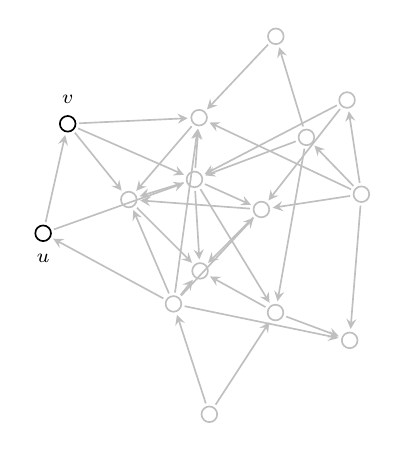
\begin{tikzpicture}[
  -stealth,
  shorten < = 1pt,
  shorten > = 1pt,
  semithick,
  font = \scriptsize,
  background default draw = black,
  background draw = lightgray,
  draw on = <3->,
  every node/.style = {
    draw, 
    circle,
    inner sep = 2pt
  }
  ]
  \node (0) at (3.090, 0.500) {};
  \node (1) at (5.021, 3.295) {};
  \node (2) at (4.839, 4.491) {};
  \node (3) at (2.634, 1.902) {};
  \node (4) at (4.323, 4.017) {};
  \node [background draw = black] (5) at (0.979, 2.799) {};
  \node [visible on = <3->, below = 0pt of 5, draw = none] {$u$};
  \node (6) at (3.934, 5.300) {};
  \node [background draw = black] (7) at (1.291, 4.189) {};
  \node [visible on = <3->, above = 0pt of 7, draw = none] {$v$};
  \node (8) at (2.901, 3.483) {};
  \node (9) at (2.960, 4.267) {};
  \node (10) at (3.751, 3.101) {};
  \node (11) at (3.930, 1.792) {};
  \node (12) at (2.067, 3.227) {};
  \node (13) at (4.872, 1.439) {};
  \node (14) at (2.972, 2.321) {};

  \draw (0) -- (3);
  \draw <-1> (0) -- (11);
  \draw (1) -- (2);
  \draw (1) -- (4);
  \draw <-1> (1) -- (9);
  \draw (1) -- (10);
  \draw <-1> (1) -- (13);
  \draw (2) -- (8);
  \draw (2) -- (10);
  \draw <-1> (3) -- (5);
  \draw <-1> (3) -- (9);
  \draw <-1> (3) -- (10);
  \draw (3) -- (12);
  \draw (3) -- (13);
  \draw <-1> (3) -- (14);
  \draw <-1> (4) -- (6);
  \draw (4) -- (8);
  \draw <-1> (4) -- (11);
  \draw <-1> (5) -- (7);
  \draw (5) -- (8);
  \draw (6) -- (9);
  \draw (7) -- (8);
  \draw <-1> (7) -- (9);
  \draw <-1> (7) -- (12);
  \draw <-1> (8) -- (9);
  \draw <-1> (8) -- (10);
  \draw <-1> (8) -- (11);
  \draw (8) -- (12);
  \draw (8) -- (14);
  \draw <-1> (9) -- (12);
  \draw (10) -- (12);
  \draw (10) -- (14);
  \draw (11) -- (13);
  \draw (11) -- (14);
  \draw <-1> (12) -- (14);
\end{tikzpicture}

    \end{column}
  \end{columns}
\end{frame}

\subsection{Link Prediction as an Embedding Problem}
\begin{frame}{Link Prediction as an Embedding Problem}
  \begin{itemize}
    \item An \emph{embedding} is a representation of one mathematical structure in the terms of another, e.g.\ \emph{graphs} represented as \emph{vectors}.
  \end{itemize}
\end{frame}

\begin{frame}{Link Prediction as an Embedding Problem}{Learning Embeddings}
  \begin{columns}
    \begin{column}{0.5 \textwidth}
      \centering
      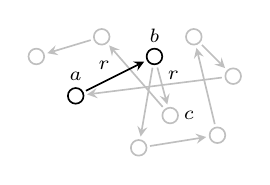
\begin{tikzpicture}[
    -stealth,
    semithick,
    shorten < = 1pt,
    shorten > = 1pt,
    font = \scriptsize,
    background default draw = black,
    background draw = lightgray,
    every node/.style = {
        circle,
        inner sep = 2pt,
        background default draw = black,
        background draw = lightgray,
      }
  ]
  \node (a) at (0, 0) [draw = black] {};
  \node (aa) [draw = none, inner sep = 0pt, above = 1pt of a, visible on = <2->] {$a$};
  \node (b) at (1, 0.5) [draw = black] {};
  \node (bb) [draw = none, inner sep = 0pt, above = 1pt of b, visible on = <2->] {$b$};
  \node (c) at (1.2, -0.25) [draw on = <2-3>] {};
  \node (cc) [draw = none, inner sep = 0pt, right = 1pt of c, visible on = <4->] {$c$};
  \node (d) at (0.8, -0.66) [draw on = <2->] {};
  \node (e) at (0.33, 0.75) [draw on = <2->] {};
  \node (f) at (-0.5, 0.5) [draw on = <2->] {};
  \node (g) at (2, 0.25) [draw on = <2->] {};
  \node (h) at (1.8, -0.5) [draw on = <2->] {};
  \node (i) at (1.5, 0.75) [draw on = <2->] {};

  \draw [draw on = <2->] (c) -- (e);
  \draw [draw on = <2->] (e) -- (f);
  \draw [draw on = <2->] (b) -- (d);
  \draw [draw on = <2->] (d) -- (h);
  \draw [draw on = <2->] (h) -- (i);
  \draw [draw on = <2->] (i) -- (g);
  \draw [draw on = <2->] (g) -- (a);
  \draw [draw = black] (a) -- node [draw = none, auto, visible on = <3->] {$r$} (b);
  \draw [draw on = <2-3>] (b) -- node [draw = none, auto, visible on = <4->] {$r$} (c);
\end{tikzpicture}

    \end{column}
    \begin{column}{0.5 \textwidth}
      \centering
      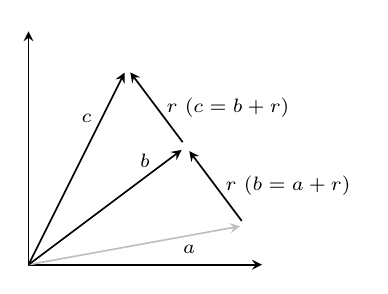
\begin{tikzpicture}[-stealth, shorten < = 1pt, shorten > = 1pt, draw = black, semithick, font = \scriptsize]
  \node (a) at (2.75, 0.5) [inner sep = 0pt] {};
  \node (b) at (2.0, 1.5) [inner sep = 0pt] {};
  \node (c) at (1.25, 2.5) [inner sep = 0pt] {};

  \draw [stealth-stealth] (0, 3) -- (0, 0) -- (3, 0);

  \draw [visible on = <3-4>] (a) -- node [auto, right] {$r$ ($b = a + r$)} (b);
  \draw [visible on = <5->] (b) -- node [auto, right] {$r$ ($c = b + r$)} (c);

  \draw <2-> [shorten < = 0pt, background default draw = black, background draw = lightgray, draw on = <5->] (0, 0) -- node [near end, below] {$a$} (a);
  \draw <2-> [shorten < = 0pt] (0, 0) -- node [near end, above] {$b$} (b);
  \draw <6-> [shorten < = 0pt] (0, 0) -- node [near end, left] {$c$} (c);
\end{tikzpicture}

    \end{column}
  \end{columns}
\end{frame}

\begin{frame}{Link Prediction as an Embedding Problem}{Inferring with Embeddings}
  \begin{columns}
    \begin{column}{0.6 \textwidth}
      \begin{itemize}[<+->]
        \item Are $d$ and $a$ related with $r$? \onslide<3->{Probably not!}
        \item We use the distance 
          \[(d + r) - a\]
          as plausibility measure.
      \end{itemize}
    \end{column}
    \begin{column}{0.4 \textwidth}
      \centering
      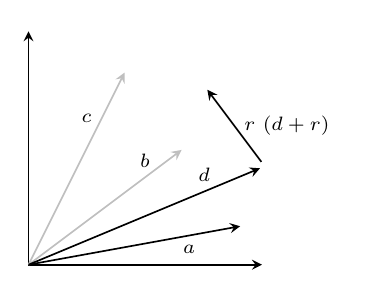
\begin{tikzpicture}[-stealth, shorten < = 1pt, shorten > = 1pt, draw = black, semithick, font = \scriptsize]
  \node (a) at (2.75, 0.5) [inner sep = 0pt] {};
  \node (b) at (2.0, 1.5) [inner sep = 0pt] {};
  \node (c) at (1.25, 2.5) [inner sep = 0pt] {};
  \node (d) at (3, 1.25) [inner sep = 0pt] {};

  \draw [stealth-stealth] (0, 3) -- (0, 0) -- (3, 0);

  \draw [shorten < = 0pt] (0, 0) -- node [near end, below] {$a$} (a);
  \draw [draw = lightgray, shorten < = 0pt] (0, 0) -- node [near end, above] {$b$} (b);
  \draw [draw = lightgray, shorten < = 0pt] (0, 0) -- node [near end, left] {$c$} (c);
  \draw [shorten < = 0pt] (0, 0) -- node [near end, above] {$d$} (d);
  \draw [visible on = <2->] (d) -- node [midway, right] {$r$ ($d + r$)} ++(-0.75, 1);
\end{tikzpicture} 

    \end{column}
  \end{columns}
\end{frame}

\subsection{Embedding Hierarchies}
\begin{frame}{Link Prediction as an Embedding Problem}{Embedding Semantic Hierarchies}
  \begin{itemize}
    \item<+-> Hierarchy-Aware Knowledge Graph Embedding (HAKE)
    \item<+-> Knowledge naturally exhibits hierarchies.
    \item<+-> Polar coordinates help encode entities on different hierarchical levels.
      \begin{columns}<.->
        \begin{column}{0.5 \textwidth}
          \centering
          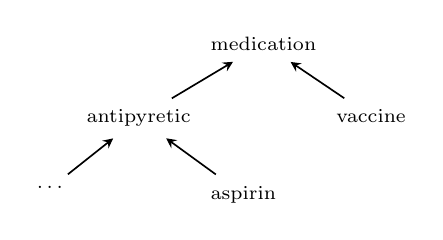
\begin{tikzpicture}[font = \scriptsize, -stealth, semithick, shorten < = 1pt, shorten > = 1pt, draw = black]
  \node (medication) {medication};
  \node (antipyretic) [below left = 0.5cm and 0cm of medication] {antipyretic};
  \node (aspirin) [below right = 0.5cm and 0cm of antipyretic] {aspirin};
  \node (a) [below left = 0.5cm and 0cm of antipyretic] {\dots};
  \node (vaccine) [below right = 0.5cm and 0cm of medication] {vaccine};

  \draw (antipyretic) -- (medication);
  \draw (aspirin) -- (antipyretic);
  \draw (vaccine) -- (medication);
  \draw (a) -- (antipyretic);
\end{tikzpicture}

        \end{column}
        \begin{column}{0.5 \textwidth}
          \centering
          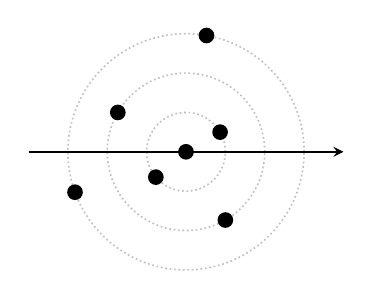
\begin{tikzpicture}[semithick, font = \scriptsize, label distance = 0pt, every node/.style = { inner sep = 2pt, circle, fill }]
  \draw [densely dotted, draw = lightgray] (0, 0) circle (0.5);
  \draw [densely dotted, draw = lightgray] (0, 0) circle (1);
  \draw [densely dotted, draw = lightgray] (0, 0) circle (1.5);
  \draw [-stealth, draw = black] (-2, 0) -- (2, 0);

  \node (medication) at (0, 0) {};
  \node (antipyretic) at (30:0.5) {};
  \node (vaccine) at (220:0.5) {};
  \node (aspirin) at (150:1) {};
  \node (a) at (300:1) {};
  \node (b) at (200:1.5) {};
  \node (c) at (80:1.5) {};
\end{tikzpicture}

        \end{column}
      \end{columns}
    \item<+-> Hierarchies are not explicitly embedded but a consequence of the approach. 
  \end{itemize}
\end{frame}

\section{Experiment Results}
\begin{frame}{Experiment Results}
  \begin{itemize}[<+->]
    \item Replication: $0.172\%$ to $-11.7\%$ deviation.
    \item Domain-specific data: close to $50\%$ of replication performance (at best).
  \end{itemize}
\end{frame}

\subsection{Visualising Embeddings}
\begin{frame}{Experiment Results}{Visualising Embeddings}
  \begin{columns}[b]
    \begin{column}{0.5 \textwidth}
      \begin{figure}
        \centering
        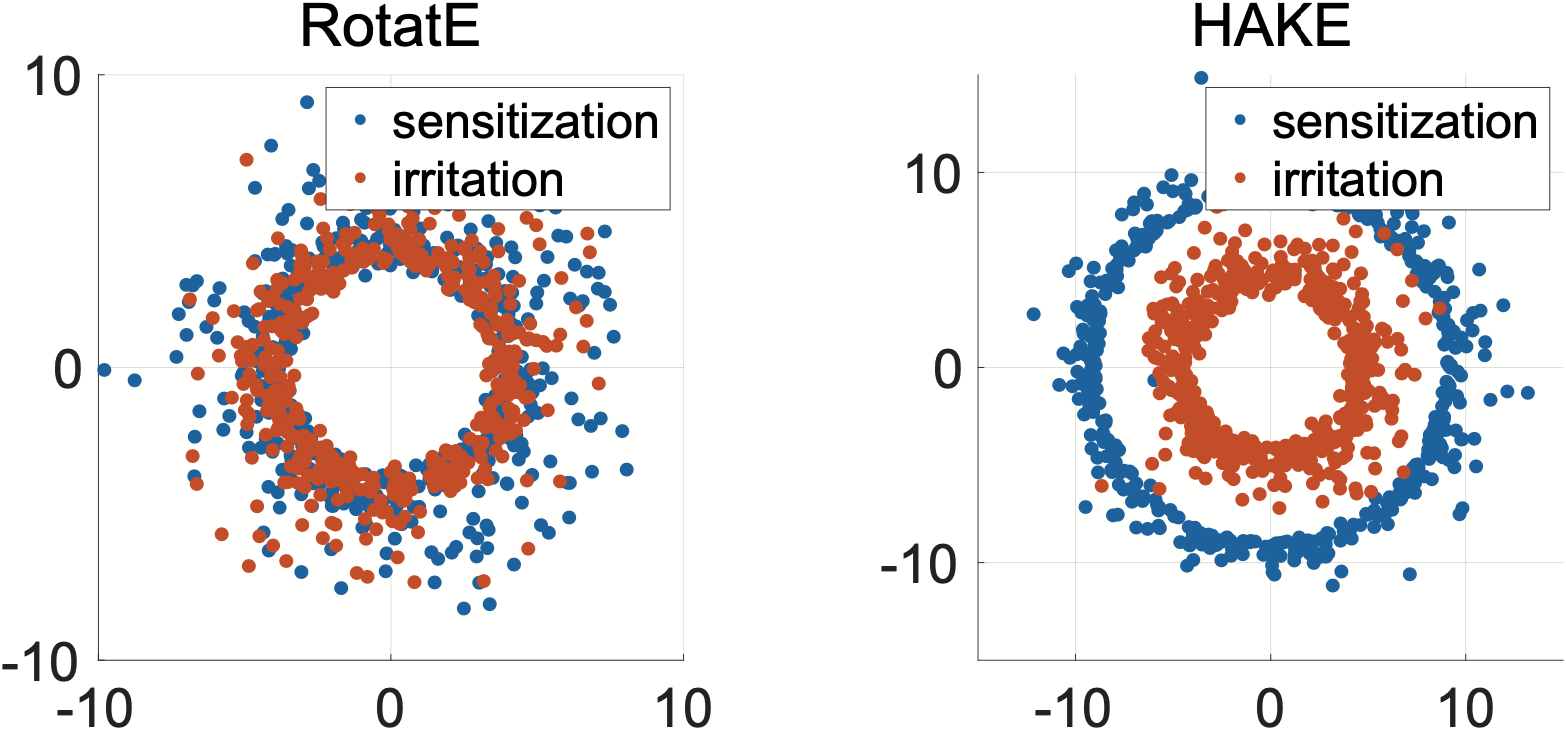
\includegraphics[width = 1 \textwidth]{figures/hake-plots.png}
        \caption{HAKE Paper}
      \end{figure}
    \end{column}

    \begin{column}{0.5 \textwidth}
      \begin{figure}
        \centering
        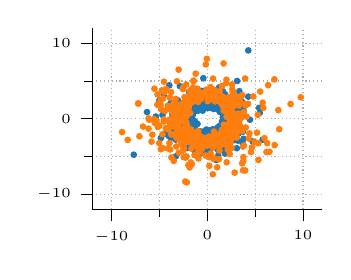
\begin{tikzpicture}[-, font = \tiny]
  \definecolor{color0}{rgb}{0.12156862745098,0.466666666666667,0.705882352941177}
  \definecolor{color1}{rgb}{1,0.498039215686275,0.0549019607843137}

  \begin{axis}[
    tick align=outside,
    tick pos=left,
    axis lines*=left,
    x grid style={white!69.0196078431373!black},
    xmin=-12, xmax=12,
    xtick style={color=black},
    y grid style={white!69.0196078431373!black},
    ymin=-12, ymax=12,
    ytick style={color=black},
    width = 4.5cm,
    mark size = 1pt,
    grid=both,
    grid style=densely dotted,
    minor tick num = 1,
    ]
    \addplot [only marks, mark=*, draw=color0, fill=color0, colormap/viridis]
      table{%
        x                      y
        0.674351751804352 1.30242300033569
        1.50970387458801 1.34348547458649
        -1.45299386978149 -1.13374543190002
        -0.329412162303925 3.63854575157166
        2.15575671195984 -1.46235072612762
        0.0572933033108711 3.29225707054138
        2.36535954475403 1.18888652324677
        -0.644977748394012 1.81655955314636
        1.29007136821747 1.02680575847626
        -3.32160639762878 0.115652106702328
        -0.789286911487579 2.36524796485901
        0.307487457990646 2.81262683868408
        2.14750146865845 1.32985651493073
        1.31883156299591 0.917830228805542
        -2.02439785003662 1.30371737480164
        0.667751252651215 2.15133452415466
        -2.15937852859497 1.83368396759033
        2.32770180702209 -0.800995707511902
        -0.0246539246290922 -2.41804265975952
        0.430213838815689 -2.35427737236023
        -1.32584059238434 -1.16411435604095
        -1.05717527866364 3.61925005912781
        -0.212821960449219 -3.71537852287292
        0.339982241392136 -2.19166326522827
        0.489246517419815 2.34129333496094
        -0.767160296440125 -2.22586870193481
        1.45977032184601 1.05145490169525
        1.21666073799133 1.44527232646942
        2.62477660179138 1.53766775131226
        -1.64476668834686 -3.44075155258179
        3.09224939346313 -3.90381979942322
        -4.43400192260742 -1.99670028686523
        -2.13069105148315 -1.30508434772491
        -2.82940649986267 -0.238278672099113
        -1.39121842384338 -0.981843948364258
        -1.07351088523865 1.68256497383118
        -2.03602719306946 -0.487134993076324
        0.411348968744278 3.73512601852417
        0.617938995361328 2.74811363220215
        0.248999610543251 -1.95602250099182
        -0.0843510851264 2.04418039321899
        1.69428324699402 0.272302210330963
        -0.296751350164413 2.29928088188171
        0.606043219566345 1.44542837142944
        -1.12327170372009 1.59369957447052
        -2.83481073379517 -1.10467100143433
        -2.51442766189575 -1.09406304359436
        -0.873412311077118 3.07123041152954
        2.19000172615051 -0.529131889343262
        -1.43793404102325 3.42490434646606
        3.73219323158264 0.576773881912231
        -1.8958375453949 2.07611203193665
        1.60314512252808 -0.671844601631165
        -2.33243656158447 1.46089136600494
        0.39659795165062 3.54472947120667
        3.14550065994263 0.174216508865356
        -2.00382280349731 0.91193288564682
        1.6359326839447 1.00882387161255
        -2.01002502441406 0.382571488618851
        -3.28928828239441 -1.85040938854218
        -1.29606235027313 -1.77962958812714
        -1.96118605136871 1.76579761505127
        -6.28650426864624 0.891581237316132
        1.46217978000641 -1.33745980262756
        -5.00297594070435 2.42195916175842
        -1.71834921836853 2.35929751396179
        -0.714460551738739 1.77828991413116
        -0.396960079669952 -2.55753755569458
        0.455569267272949 -2.21655678749084
        0.820585131645203 -2.98431015014648
        2.84520173072815 1.39759969711304
        1.88483285903931 -1.73819077014923
        1.55124282836914 -2.24502778053284
        -1.54208409786224 0.857647716999054
        -0.0930347591638565 -4.4599757194519
        -1.29272377490997 -0.325635671615601
        -3.59374618530273 0.875617444515228
        1.31803047657013 -0.990396738052368
        -0.450012892484665 2.07954359054565
        -1.23279702663422 3.49819827079773
        -1.72823989391327 -0.379563421010971
        -3.29138135910034 -2.75603842735291
        -0.511855065822601 2.42980098724365
        -0.0349343381822109 -2.23152732849121
        -0.941066741943359 -1.79137861728668
        2.83780097961426 0.427334874868393
        2.49536299705505 1.59894442558289
        -2.22815871238708 0.669797241687775
        1.93174421787262 -0.250525265932083
        -2.20547771453857 0.509948015213013
        0.349134683609009 -3.62919044494629
        0.617802560329437 1.82705557346344
        0.00282687996514142 3.38554263114929
        1.53477811813354 -0.386467456817627
        0.025955630466342 -1.84299373626709
        1.12899696826935 1.50993537902832
        1.63244450092316 3.65720677375793
        -4.50099420547485 -2.01381850242615
        2.61137175559998 -0.913346827030182
        -2.54289817810059 -0.981023132801056
        -2.23151826858521 0.173626750707626
        -1.92252099514008 -1.48797643184662
        -0.170799016952515 1.69050574302673
        3.17792272567749 0.478481620550156
        1.93503761291504 -0.694665253162384
        2.4980480670929 -0.278414696455002
        -1.01312863826752 -0.685770153999329
        0.171704709529877 -2.3221423625946
        1.1440577507019 -4.87651062011719
        1.18330228328705 -1.74444973468781
        1.7557315826416 0.952545642852783
        1.59275960922241 -4.05061817169189
        -2.4807596206665 1.16238045692444
        1.35274994373322 1.35547637939453
        1.6399450302124 0.645010054111481
        -1.72433924674988 -1.84551382064819
        4.29286909103394 9.0551290512085
        -0.152346685528755 3.79717993736267
        -2.08617687225342 -0.511158883571625
        -3.26575613021851 2.24550604820251
        -2.15495586395264 0.259006887674332
        0.183513075113297 -2.39810037612915
        -0.611124753952026 -2.12998366355896
        0.0802273824810982 -2.25636434555054
        1.18051302433014 3.67018485069275
        1.74754106998444 1.95274829864502
        1.27508306503296 -2.6106379032135
        1.58193802833557 -1.23122429847717
        0.274746924638748 2.05359959602356
        1.68117332458496 0.940564095973969
        -0.626959323883057 1.80775713920593
        2.72647023200989 2.21431016921997
        1.95830202102661 -0.385492414236069
        -0.173520520329475 -2.78126430511475
        -2.07899832725525 -1.83876633644104
        1.99604773521423 0.135446980595589
        1.041384100914 -2.18570780754089
        -1.89104664325714 -0.85527628660202
        -3.03910040855408 -0.859738886356354
        -2.90987253189087 -0.654278039932251
        0.223095282912254 -4.36389446258545
        2.74295234680176 -0.188321217894554
        -1.10224914550781 1.71840476989746
        -2.26515412330627 -1.48696005344391
        0.385700970888138 2.20935702323914
        0.675397276878357 -1.94993698596954
        2.51516723632812 0.619122207164764
        1.83570683002472 -3.29619359970093
        1.43442213535309 -3.33121299743652
        -4.52566242218018 3.14609336853027
        2.7626473903656 0.960769534111023
        2.80473613739014 1.38084924221039
        5.41573238372803 1.44528949260712
        1.99674487113953 -4.0225625038147
        0.440433889627457 2.91793966293335
        -1.95281052589417 2.18929934501648
        1.20067429542542 1.92063319683075
        -0.970863461494446 -2.50849556922913
        -1.98082661628723 1.29522824287415
        1.93634605407715 0.732313275337219
        -0.645637392997742 3.70057320594788
        1.88178563117981 0.657862663269043
        -2.32559466362 0.373833179473877
        2.87445402145386 1.24673318862915
        -1.63720512390137 -0.378566294908524
        -2.33545446395874 -3.01327657699585
        -0.13149493932724 2.30311584472656
        -2.58492636680603 1.51384627819061
        -1.35840535163879 -2.1828510761261
        2.03640532493591 1.56503891944885
        2.5219783782959 -1.97711718082428
        -2.2682511806488 -5.11103343963623
        1.81962466239929 0.754550516605377
        0.864357471466064 -3.82420134544373
        -1.60365891456604 -2.24768567085266
        0.92453944683075 2.06269598007202
        1.94212985038757 -1.15116894245148
        1.96622288227081 0.0894124880433083
        0.304690569639206 2.15562081336975
        -0.291741371154785 2.96998763084412
        2.51924157142639 0.226068377494812
        1.61938464641571 -1.46599662303925
        -1.52265846729279 3.11520671844482
        -1.42123508453369 -1.85895931720734
        1.37268686294556 -2.70752143859863
        2.91116690635681 -2.01681876182556
        -2.08059859275818 1.01222121715546
        1.53716433048248 1.53740859031677
        0.339727580547333 -1.78124535083771
        -2.20847702026367 0.698060870170593
        -1.76045858860016 1.23193597793579
        -3.0255811214447 -0.612332701683044
        -1.18681740760803 -3.79063320159912
        -2.07859706878662 0.940325200557709
        1.61221671104431 -2.65262413024902
        -1.52444612979889 2.53642058372498
        1.61708796024323 -1.94024288654327
        -2.65545153617859 -3.12909412384033
        -2.34134936332703 -1.1531366109848
        3.1245448589325 5.00672578811646
        1.12124395370483 -1.32157099246979
        2.4456262588501 -3.92400813102722
        -2.15849256515503 -0.495442122220993
        0.054987758398056 1.41979646682739
        1.90560925006866 0.367669284343719
        2.24440836906433 -1.87487292289734
        1.30217909812927 -1.05078363418579
        -0.93597012758255 1.36152970790863
        -0.196055337786674 -2.17717337608337
        -2.18415403366089 2.13177704811096
        -4.84101390838623 -2.55875205993652
        2.1652238368988 -0.486549854278564
        -2.13110303878784 -3.88149642944336
        -2.15195369720459 0.18650096654892
        2.7499144077301 2.78155636787415
        2.66842293739319 1.80188584327698
        -1.80620932579041 1.23889684677124
        1.61507833003998 -1.07863461971283
        1.46756398677826 1.5929229259491
        -3.03694629669189 0.141359075903893
        0.569444835186005 2.98254132270813
        -2.00337028503418 2.34776973724365
        0.368226647377014 -2.2118604183197
        -1.21481132507324 -4.337486743927
        1.32894670963287 -1.7718186378479
        3.36957573890686 -0.128571346402168
        -2.83322286605835 0.0902491062879562
        -3.39244365692139 -1.90781104564667
        -3.82191729545593 2.08197355270386
        1.84026730060577 -1.56757867336273
        -2.07794404029846 -0.556463420391083
        2.72636246681213 -0.830195963382721
        3.16763520240784 1.18697452545166
        0.939878880977631 -5.46400356292725
        2.63294839859009 -0.250868052244186
        0.391123175621033 -1.85919189453125
        3.53665494918823 0.192690566182137
        0.298664152622223 -2.53323984146118
        1.85894179344177 -4.61908769607544
        -0.65016508102417 -3.77154898643494
        -3.07846927642822 2.46924614906311
        0.0788464620709419 -3.55508065223694
        2.68543601036072 3.50706601142883
        -2.60688328742981 -1.72310304641724
        2.28833603858948 1.55942916870117
        0.741317689418793 -2.84565997123718
        1.73700475692749 -1.82228291034698
        0.561797380447388 3.43332242965698
        2.68443703651428 0.171571895480156
        2.03061628341675 2.92162775993347
        -1.73877239227295 -2.2331862449646
        -1.37865602970123 -1.87913680076599
        -3.35551261901855 -0.737092018127441
        0.390743285417557 -2.43885254859924
        -2.50679683685303 -2.35738825798035
        0.049151673913002 2.38249826431274
        2.95269632339478 1.6264922618866
        1.16492986679077 3.08081340789795
        -0.662126958370209 -2.1804838180542
        1.68034589290619 0.987772762775421
        3.30448293685913 -1.89993107318878
        3.82102513313293 1.80606520175934
        2.20380783081055 -1.92721939086914
        -2.1527898311615 -1.10486829280853
        -1.42894196510315 2.10545492172241
        -3.23879599571228 0.08809644728899
        0.629426896572113 -2.62016940116882
        2.83130407333374 -2.17989945411682
        -1.21643972396851 -1.75109100341797
        1.4410959482193 1.7272162437439
        2.07166981697083 2.60808897018433
        1.40251302719116 -4.12457370758057
        -1.60669565200806 0.0432073809206486
        -3.4449896812439 -0.564860880374908
        0.164817899465561 -1.527428150177
        -2.85226941108704 4.32855129241943
        -0.356214612722397 2.27512669563293
        -0.117734298110008 2.65855526924133
        3.66673707962036 -3.14825677871704
        1.02279829978943 1.29724836349487
        -2.15994501113892 1.73434579372406
        2.11049127578735 0.558534562587738
        1.76048445701599 -0.263418525457382
        -3.28632664680481 -1.18294775485992
        -2.24060606956482 0.808234989643097
        2.34073090553284 0.305641323328018
        4.73615217208862 -3.00352025032043
        2.21820569038391 0.0273949690163136
        -3.2793276309967 -4.97785902023315
        -2.08523082733154 1.77418267726898
        -1.59333372116089 -0.105179592967033
        -0.438859939575195 1.60914850234985
        0.360082149505615 -1.88192927837372
        -1.77391290664673 -1.77503764629364
        -2.91240692138672 0.624114990234375
        1.5506294965744 2.01639151573181
        4.46548271179199 -0.122123397886753
        -0.871042430400848 -1.98256719112396
        -0.406230539083481 5.37528324127197
        0.735697329044342 -1.65818977355957
        3.08075571060181 -0.560038089752197
        -2.41618037223816 0.82501232624054
        0.793899476528168 -2.86187958717346
        -3.80871248245239 -2.54954981803894
        -1.40158677101135 -2.89373660087585
        5.48933410644531 0.782140731811523
        1.69929325580597 -2.0677125453949
        3.19785523414612 -2.89516830444336
        0.040493194013834 2.10921764373779
        2.93175983428955 1.68314445018768
        2.68328309059143 -0.292267173528671
        -0.231271013617516 -2.0463662147522
        0.932951092720032 -1.40121030807495
        0.631666362285614 2.42450594902039
        -3.6424663066864 0.609528660774231
        -3.36168432235718 -1.82312428951263
        3.60522127151489 2.31295871734619
        2.04682159423828 0.208842560648918
        -1.66949820518494 -1.32706069946289
        1.19212257862091 3.09021306037903
        -1.52479732036591 -0.93670654296875
        1.85490965843201 0.376823723316193
        -4.05087804794312 -2.24440789222717
        2.68894290924072 -0.25838229060173
        2.75908493995667 2.60114073753357
        2.20211577415466 1.92574679851532
        2.80530714988708 -2.83271193504333
        1.54051756858826 1.59565198421478
        1.37744069099426 1.14519441127777
        3.79773187637329 -2.66147947311401
        -3.95549201965332 4.42928838729858
        2.3581120967865 -2.80697560310364
        -1.05521464347839 3.41798043251038
        -1.24358153343201 1.80476367473602
        1.2132602930069 1.99974811077118
        -1.40552890300751 1.21030938625336
        0.851368129253387 3.68970346450806
        -2.05195426940918 1.27248728275299
        2.317946434021 -0.615121841430664
        0.551553010940552 -3.69386863708496
        1.598761677742 -2.33865332603455
        2.60761880874634 0.679990172386169
        0.0671623423695564 2.24471139907837
        -3.29137921333313 0.439654380083084
        0.388652354478836 3.20428252220154
        -2.46205973625183 1.47697114944458
        -1.9947098493576 1.89264810085297
        1.73364448547363 -1.04079174995422
        2.6735098361969 -2.41500759124756
        2.13323998451233 1.12404596805573
        -0.330389022827148 -2.21714019775391
        1.1217006444931 -1.11742162704468
        1.68981444835663 2.27323508262634
        -1.26467776298523 1.53234803676605
        1.12185573577881 -4.1184139251709
        -0.213663175702095 2.5387442111969
        -2.32777881622314 1.91235864162445
        1.9020928144455 -2.22568726539612
        -1.83464014530182 1.17337238788605
        2.375643491745 0.482321083545685
        -1.24712538719177 0.99322110414505
        0.360436290502548 -2.5250358581543
        1.86764097213745 3.24440693855286
        -1.61804735660553 -0.25277578830719
        -1.24787664413452 1.9005651473999
        -2.0711989402771 -1.35983228683472
        -0.554239332675934 -3.13266015052795
        0.31002938747406 -4.00414276123047
        -1.43494975566864 -4.09587049484253
        -2.77164435386658 -1.19059944152832
        -3.06076049804688 -1.73145639896393
        1.91430628299713 0.00538858864456415
        -1.94709408283234 1.41922771930695
        1.39140129089355 2.54447412490845
        -0.455897808074951 -2.91713666915894
        -0.912107825279236 -2.6488630771637
        -1.24141192436218 2.14132261276245
        0.0775944665074348 1.67954814434052
        -1.93932008743286 -0.466060817241669
        -1.4183406829834 1.97276079654694
        -7.67055368423462 -4.76552152633667
        1.69875836372375 0.0733085125684738
        1.2420881986618 4.14551067352295
        2.66597700119019 -1.49980878829956
        1.57614481449127 -1.57152557373047
        0.266829669475555 -2.21425771713257
        -3.84324884414673 -0.994155645370483
        1.39879024028778 -1.18697714805603
        -1.89412176609039 3.55680465698242
        1.87528681755066 -0.148914784193039
        1.21554172039032 2.47153854370117
        -2.88505792617798 1.20384621620178
        -3.77528119087219 -2.36250758171082
        -2.86468720436096 -0.947155356407166
        3.35873246192932 3.65846014022827
        -1.02763903141022 2.18051195144653
        1.44378864765167 1.29686439037323
        -2.56537866592407 1.01579451560974
        -1.90973019599915 -0.264629244804382
        1.41443610191345 -1.70892250537872
        0.85871285200119 3.17438077926636
        -1.68156957626343 -1.39901959896088
        1.60787725448608 3.22701239585876
        -2.15234446525574 1.56458878517151
        0.125188782811165 1.5818727016449
        -0.741322159767151 2.29087257385254
        1.68313229084015 0.372123390436172
        2.27744150161743 -1.35506248474121
        -1.51590669155121 0.470446825027466
        3.77858257293701 1.19100773334503
        -2.33926200866699 -0.334868520498276
        -3.77328729629517 -1.14570212364197
        -1.9313405752182 0.849353432655334
        -2.07215213775635 0.099639393389225
        0.468930780887604 1.53912210464478
        0.507794559001923 -2.07976174354553
        1.29837918281555 -0.969516515731812
        1.9538117647171 -1.79590749740601
        -0.711705923080444 -1.67052316665649
        -1.49168610572815 0.830038726329803
        1.04447865486145 -1.54920482635498
        1.69817769527435 -2.49227952957153
        0.0386521369218826 1.73179888725281
        -2.6880247592926 1.13260018825531
        -0.0478260591626167 2.7572968006134
        0.136913746595383 -2.81842637062073
        1.05656385421753 3.57793855667114
        -2.01499629020691 -0.259242981672287
        -3.22104024887085 -0.173477903008461
        0.92283022403717 1.56806218624115
        -4.6670880317688 0.496757596731186
        -2.66206288337708 0.149105429649353
        -0.338715612888336 -1.67574620246887
        0.297347396612167 2.1216402053833
        -0.996773838996887 1.04953706264496
        -2.15386414527893 0.968259871006012
        0.119176469743252 2.26562833786011
        -5.36779928207397 0.295168310403824
        -3.32902956008911 -2.4847240447998
        -2.15577912330627 -0.41963854432106
        1.34767663478851 2.45081758499146
        -0.473304748535156 1.06801617145538
        1.79994881153107 1.06995165348053
        3.04705572128296 1.08184278011322
        5.78803110122681 -2.77142071723938
        0.350184619426727 1.45068776607513
        0.597387909889221 -1.37966442108154
        1.72480988502502 -1.37516629695892
        3.27342867851257 -1.80175685882568
        1.76792073249817 -2.96711373329163
        -2.21369028091431 0.988730251789093
        -3.17030692100525 1.72633469104767
        0.826597690582275 1.8446261882782
        -3.74665451049805 -0.300996482372284
        3.70537996292114 -1.73209261894226
        -1.92982745170593 -2.48279929161072
        1.84106433391571 1.71663880348206
        2.94381523132324 0.313170194625854
        -1.61464059352875 0.0631378889083862
        -3.10743236541748 1.80536222457886
        -1.58941209316254 -1.88813424110413
        2.07362580299377 0.405246168375015
        -0.503515303134918 1.97844624519348
        1.64705109596252 -1.29611718654633
        2.60882091522217 0.918895125389099
        1.63001644611359 0.200636923313141
        -0.386273235082626 -2.54143762588501
        -2.05817675590515 2.68616509437561
        1.93088400363922 0.635994493961334
        -0.202094838023186 -2.4206702709198
        -0.101067572832108 -2.01981377601624
        -0.0870537087321281 -1.42844760417938
        -0.700562059879303 -4.56492519378662
        -1.4748831987381 2.79783153533936
        0.889686763286591 -1.98208940029144
        1.99030554294586 1.76147186756134
        -2.11591935157776 1.07134747505188
        1.89781033992767 0.891111612319946
        -1.25319635868073 -2.89034008979797
        2.98461079597473 1.05350065231323
        1.57096755504608 0.973093330860138
        -0.0161320921033621 -2.29736185073853
        0.855305075645447 2.70808792114258
        -0.223417058587074 1.87757921218872
        -2.61681365966797 1.85629057884216
        1.07849633693695 1.67803633213043
        1.54476809501648 -1.12193739414215
        -4.02429580688477 1.38566267490387
        -1.4324985742569 -2.18062376976013
        -1.45192289352417 1.13868844509125
        1.91803455352783 1.14938187599182
        1.18110942840576 1.51078033447266
        2.90945315361023 -0.373053222894669
        4.28136873245239 2.9360237121582
        -1.28974771499634 1.16232872009277
        1.13273942470551 -3.61695241928101
        -3.8605899810791 -1.2842652797699
        1.81440901756287 1.41910326480865
        -2.78209900856018 -0.130160331726074
        -1.6920975446701 -0.879405975341797
      };
    \addplot [only marks, mark=*, draw=color1, fill=color1, colormap/viridis]
      table{%
        x                      y
        -2.97603750228882 -4.49860239028931
        -0.0172200202941895 3.57849597930908
        0.196253299713135 -2.36519336700439
        -1.80555963516235 -3.0174720287323
        3.10379028320312 -1.83392584323883
        -1.76436328887939 3.80080986022949
        -2.26883888244629 -0.910714566707611
        -0.568458557128906 -3.46597814559937
        -0.0518024601042271 3.85579776763916
        -1.91920900344849 1.50736093521118
        -2.42110633850098 -1.52100145816803
        -0.939807236194611 3.59904623031616
        -4.13069438934326 1.69660127162933
        -2.60897493362427 -2.09362530708313
        0.601900398731232 -3.78640985488892
        2.68864130973816 0.582375526428223
        0.433514207601547 3.34027075767517
        1.28267514705658 2.59630155563354
        2.32405138015747 -2.28027296066284
        -0.134692996740341 -2.55520248413086
        -0.773354887962341 -2.60324048995972
        -0.147594317793846 7.20102214813232
        2.79891514778137 -1.1271276473999
        2.42383170127869 -3.16439628601074
        -4.45628356933594 3.52140665054321
        0.899726152420044 -2.96163892745972
        -2.75683760643005 -0.0495170764625072
        -2.5710985660553 0.437518417835236
        -2.45788741111755 -5.08688259124756
        -6.70514583587646 -1.03197145462036
        -3.01281547546387 -0.787461757659912
        7.43243074417114 1.14970707893372
        -3.16085338592529 4.96610593795776
        -2.43693137168884 4.25313901901245
        1.45746386051178 -2.28273105621338
        0.553736925125122 -3.06291699409485
        2.03396010398865 -5.7646861076355
        -4.67044591903687 -2.04905962944031
        1.84890866279602 -1.96055340766907
        -2.30622386932373 0.330005258321762
        -2.96458387374878 -2.25683283805847
        -8.88786220550537 -1.76817572116852
        -4.53221464157104 -0.364950567483902
        -7.08179140090942 -2.31952118873596
        -1.98280215263367 1.49832725524902
        -1.62186932563782 -1.76607024669647
        6.49883031845093 -4.37613916397095
        -3.30718588829041 -0.874099791049957
        2.17269897460938 2.02039456367493
        1.98866605758667 -2.31265091896057
        -0.641340851783752 2.64160180091858
        2.75763058662415 -0.182184621691704
        -2.68440532684326 -3.33854103088379
        1.46945941448212 2.02792644500732
        -1.66193902492523 -1.44690430164337
        2.60877466201782 -0.104804538190365
        -1.70510971546173 -5.7912654876709
        -2.06157946586609 2.16196060180664
        -2.51476192474365 -1.36962890625
        -3.39610862731934 1.67334866523743
        1.75076735019684 -2.57587194442749
        -1.03727269172668 -2.95006012916565
        1.38041138648987 -2.34287667274475
        -3.56123280525208 1.498650431633
        0.741463959217072 3.35382604598999
        -0.886228203773499 -2.74208736419678
        2.59906196594238 4.54810380935669
        -3.66598272323608 0.874234318733215
        -3.2359881401062 1.48028218746185
        -1.37170147895813 2.46533417701721
        0.820368349552155 2.29652190208435
        2.19549679756165 1.26631534099579
        -1.74405717849731 2.38593196868896
        2.43120431900024 -0.664980471134186
        4.02712774276733 -1.16215789318085
        4.66400623321533 -3.80925178527832
        -2.94282221794128 1.17139005661011
        -2.18866229057312 4.55272769927979
        2.72512483596802 -1.92126846313477
        0.147923156619072 -5.03787851333618
        -0.686645567417145 -2.92278289794922
        -3.10519957542419 -0.374150037765503
        2.11670875549316 -0.853915572166443
        3.17860126495361 2.53354859352112
        -0.943318963050842 -2.52749752998352
        -2.43307185173035 0.830033898353577
        0.0585651844739914 2.32540678977966
        0.60530298948288 5.32495784759521
        -2.19372034072876 -0.484985381364822
        -2.40454912185669 1.64723670482635
        -2.37898874282837 2.21610426902771
        -4.10148477554321 -1.37821483612061
        -4.30265283584595 3.94630789756775
        3.29223299026489 0.129899799823761
        -2.40219902992249 1.26092457771301
        -2.98351693153381 -2.21995615959167
        -3.22498393058777 -3.66761946678162
        -3.50894141197205 0.13077175617218
        -2.47641038894653 0.737302005290985
        1.03229165077209 -2.44098210334778
        -5.15777921676636 -1.10011851787567
        -0.223536401987076 -2.71500158309937
        2.45612716674805 -1.11981296539307
        0.0262930449098349 -3.05407428741455
        -0.0148911979049444 -3.54093861579895
        1.03794872760773 -6.42704582214355
        0.80759984254837 2.43488812446594
        1.3287672996521 -2.27566647529602
        -2.98204135894775 -0.18480783700943
        -0.364058077335358 -3.25574779510498
        2.13824391365051 2.00961875915527
        -2.49734950065613 -2.06138157844543
        1.23355305194855 2.52350640296936
        -0.909407138824463 -2.3459632396698
        -1.47816061973572 -2.33767080307007
        1.27902126312256 -4.21003103256226
        2.01893162727356 1.0465042591095
        3.31006646156311 1.75791156291962
        1.44988560676575 -3.46535539627075
        1.16738629341125 -3.52226781845093
        -0.995998740196228 2.58714461326599
        -0.790896475315094 -3.70190644264221
        5.35568332672119 -5.45516443252563
        3.61649227142334 0.214841514825821
        -3.30960392951965 0.0632617175579071
        1.8279287815094 -3.11058592796326
        -2.0581169128418 -1.06584095954895
        -2.90010643005371 0.356378167867661
        -3.41072297096252 -2.09283542633057
        5.8618221282959 1.44901657104492
        -0.760874092578888 -4.2919979095459
        1.63530564308167 1.7034158706665
        2.67729520797729 -1.35245394706726
        0.0806405320763588 2.76102042198181
        0.724260687828064 -3.01200675964355
        -3.53312134742737 2.01167869567871
        -0.500929951667786 -3.42391347885132
        0.0305937118828297 -3.52226948738098
        0.960378527641296 2.63421416282654
        1.54832530021667 4.34933423995972
        0.492746829986572 3.52545666694641
        2.50290775299072 2.54332590103149
        -3.94237589836121 -3.22390794754028
        3.63890671730042 -1.65454816818237
        -0.845432043075562 -3.35355448722839
        -1.07554221153259 -2.88995814323425
        2.07043361663818 1.4275141954422
        2.89733457565308 -0.592474400997162
        -6.12817573547363 -1.30158650875092
        2.37295627593994 1.96413123607635
        2.14259028434753 -4.09310674667358
        -1.42968010902405 5.06362199783325
        1.69167578220367 2.77878189086914
        -3.89660358428955 2.82039856910706
        -0.341127246618271 3.49755001068115
        2.91043782234192 0.468001544475555
        3.07780957221985 -2.48937082290649
        7.04703235626221 -3.49071550369263
        0.948294639587402 -2.43133997917175
        -5.72823333740234 -2.10792946815491
        -1.96961653232574 2.74815511703491
        -1.74199044704437 -1.60297548770905
        -2.22277402877808 -5.11126041412354
        3.4057948589325 2.36564183235168
        0.690255224704742 2.81773114204407
        3.74231481552124 -6.83334732055664
        -3.7496063709259 -2.07946181297302
        9.77412796020508 2.8494393825531
        -1.70123434066772 2.13963866233826
        -3.76973438262939 3.52717900276184
        2.36115002632141 -0.406917780637741
        -1.46708559989929 -2.12517070770264
        -3.20452475547791 -2.5649631023407
        3.25839304924011 0.678260147571564
        1.84638845920563 1.15717005729675
        2.86560249328613 1.8460191488266
        1.97964763641357 4.72818517684937
        1.96511507034302 -1.76794588565826
        -0.925475180149078 -2.29910659790039
        -0.735240995883942 -2.66899061203003
        -5.01585578918457 -3.22239017486572
        -2.39550924301147 -1.68888187408447
        -4.33934879302979 -1.23853302001953
        -2.98358988761902 6.51025629043579
        -2.412757396698 -0.076456606388092
        0.763498723506927 -2.53863549232483
        0.405452817678452 -2.83492159843445
        -1.56203877925873 -2.27649331092834
        5.2811484336853 0.515921711921692
        -1.60701906681061 -6.01009845733643
        -1.80642855167389 -1.70576238632202
        2.38234877586365 -3.69409894943237
        2.95878481864929 0.323827624320984
        -0.949138522148132 2.2372465133667
        2.06851530075073 1.40473616123199
        3.96239018440247 1.9592387676239
        -2.79454278945923 -2.26703095436096
        -2.94969582557678 0.0454663895070553
        2.61825013160706 -1.40455675125122
        -5.46866655349731 -0.539813697338104
        -0.037243939936161 7.9441237449646
        0.484484523534775 2.82070446014404
        -1.66502690315247 -1.69494986534119
        -2.30277729034424 1.45260977745056
        -2.44364547729492 -3.9365062713623
        7.52247905731201 -1.38746523857117
        3.78253531455994 -5.07261228561401
        4.96411800384521 -3.08623242378235
        0.583265542984009 -7.36338186264038
        -3.29130578041077 2.62910485267639
        -1.32003605365753 -4.81552839279175
        1.71168994903564 7.33193302154541
        -5.81836032867432 -3.03345370292664
        -5.53967952728271 -0.0599229522049427
        -1.93926608562469 2.10182452201843
        4.406090259552 -1.94511353969574
        -2.03874921798706 -2.33670783042908
        3.745281457901 0.62021940946579
        3.6547999382019 -5.90986108779907
        2.39033246040344 1.04589378833771
        6.19487380981445 -4.40338563919067
        0.835368633270264 -3.34396004676819
        0.220761701464653 -6.23711013793945
        -0.912407279014587 -5.26080942153931
        -0.725049197673798 2.69806480407715
        -0.960383534431458 -1.62672698497772
        1.9327986240387 -2.09114241600037
        -2.20800471305847 2.74594378471375
        -0.753490924835205 2.7971978187561
        2.78206181526184 3.34610199928284
        -4.73699903488159 3.76638221740723
        -1.36502313613892 -3.58986616134644
        1.73669922351837 -0.778757750988007
        3.16161060333252 2.85584139823914
        -3.06243109703064 -0.424719959497452
        -2.52055835723877 -4.21494913101196
        -2.53174996376038 3.93863034248352
        2.76140880584717 -0.42247685790062
        -7.18017482757568 2.03273558616638
        4.35700130462646 -2.62529945373535
        -2.08817338943481 1.81887054443359
        -0.184178218245506 -4.86093807220459
        5.34441232681274 -3.24818420410156
        -1.96974837779999 -6.11577033996582
        0.443029761314392 -3.16829133033752
        -1.69145703315735 2.37236857414246
        -2.24643588066101 -2.35957598686218
        -1.82741284370422 -6.45127296447754
        0.411270439624786 2.62916731834412
        -3.358891248703 -0.802841067314148
        -1.77822363376617 0.752987921237946
        -1.01869404315948 3.98212385177612
        2.58108878135681 0.601783871650696
        1.44320201873779 2.33873987197876
        -4.87023448944092 1.85423362255096
        2.2963125705719 2.40378975868225
        5.98443031311035 -2.572265625
        0.166201442480087 3.05350136756897
        2.97141742706299 -1.89711225032806
        2.87434959411621 -0.963994681835175
        4.81779050827026 2.95696806907654
        -2.53277254104614 0.584366917610168
        1.64230179786682 -3.12876343727112
        -4.86076068878174 2.43631625175476
        3.83631753921509 -3.55107641220093
        -1.46319198608398 -3.47261381149292
        2.01254153251648 5.17487382888794
        2.14419150352478 -0.883749425411224
        1.66452705860138 -2.22361993789673
        -2.26537489891052 1.63144826889038
        1.34499561786652 -2.30715584754944
        3.47157979011536 -1.00136959552765
        -2.08303546905518 -1.41556644439697
        -3.1598949432373 -1.99994933605194
        -2.20872831344604 2.2219340801239
        -1.49173808097839 -1.94233274459839
        3.95443797111511 5.3383355140686
        2.86721706390381 -7.13572645187378
        -1.9172477722168 -1.78224039077759
        -1.17157137393951 -2.07973456382751
        -0.906361103057861 -2.09042191505432
        3.44980120658875 0.23329795897007
        1.61824703216553 2.3488655090332
        3.64478468894958 3.13141536712646
        -2.94213438034058 -0.466443061828613
        -2.35890889167786 1.78089642524719
        2.52981424331665 -1.28680682182312
        -7.21166944503784 2.02282238006592
        -1.66326940059662 2.89210033416748
        -2.36999464035034 2.86727285385132
        -5.20723533630371 1.87179851531982
        2.51244401931763 2.80479383468628
        -2.16064548492432 -4.98482894897461
        -5.30101346969604 -0.273205041885376
        2.93822312355042 0.391499549150467
        2.67179465293884 3.57042908668518
        5.53871202468872 3.60088872909546
        -1.54721665382385 3.83454465866089
        2.24706840515137 2.88239979743958
        1.13719737529755 -2.44800186157227
        -4.63185453414917 -3.88128113746643
        -2.10629200935364 -2.58839178085327
        -1.01220595836639 2.88942003250122
        -1.20074224472046 5.97981262207031
        2.61775970458984 3.93196702003479
        -2.37295365333557 -0.125605642795563
        -2.2889039516449 1.54966115951538
        -2.80864500999451 0.77188366651535
        -0.529658138751984 -2.61603164672852
        -1.81375777721405 3.63405990600586
        0.8129021525383 2.67627286911011
        -1.66581773757935 2.44282269477844
        -1.48292076587677 4.16605854034424
        0.975304186344147 2.51525354385376
        2.66421341896057 0.805055975914001
        -5.51130771636963 3.98495817184448
        -2.37182116508484 -1.60888266563416
        1.59710395336151 2.9494252204895
        -2.40087699890137 2.2838671207428
        6.36364889144897 4.4516863822937
        -5.18825531005859 3.22762537002563
        -3.73096537590027 -0.954808533191681
        3.00385332107544 -2.2220094203949
        2.77119898796082 -0.692945599555969
        5.79068231582642 2.13039779663086
        0.879918456077576 -2.20921611785889
        -1.14388394355774 -2.23885869979858
        0.631751656532288 -2.45787858963013
        -0.75711977481842 -2.30599474906921
        -1.5125367641449 -2.14877247810364
        -3.95009446144104 -0.460586071014404
        1.29898822307587 3.65794610977173
        2.37334275245667 -0.31124484539032
        -1.11124753952026 2.46948432922363
        -0.493759751319885 -2.51502561569214
        -4.51542329788208 4.91866540908813
        -4.01423978805542 -1.32938146591187
        4.26611280441284 1.98613321781158
        2.63945150375366 -0.339798241853714
        3.06235599517822 -1.04236972332001
        2.57024717330933 -0.63770580291748
        2.97704648971558 -0.967885136604309
        -3.78458499908447 -0.258931636810303
        -3.62629413604736 -0.883924603462219
        2.34768748283386 -4.66838216781616
        1.75496518611908 2.05988383293152
        1.52292466163635 -2.17241072654724
        2.96292781829834 0.549409449100494
        6.26184988021851 -3.23065257072449
        0.6961709856987 -1.69671487808228
        -0.462553322315216 -3.69931268692017
        2.87646675109863 2.70003318786621
        -2.309321641922 1.74879169464111
        2.74982452392578 -0.921504199504852
        3.32969307899475 -0.351338386535645
        -2.12854027748108 -8.43423748016357
        -0.778059899806976 -3.19091176986694
        0.521984934806824 2.96198225021362
        -4.07163715362549 1.44961452484131
        0.765446662902832 3.81003069877625
        2.29591155052185 -1.01942217350006
        0.763469159603119 -3.30363893508911
        -2.73455882072449 0.39808651804924
        -3.34813642501831 0.256385326385498
        0.773155927658081 -2.84058427810669
        2.73443055152893 -0.757377982139587
        1.52158749103546 -1.47985184192657
        -2.05824637413025 2.79535055160522
        -0.354844868183136 -2.83766269683838
        1.06591641902924 -2.06188893318176
        0.626585721969604 -5.30482864379883
        -2.27507185935974 1.25285732746124
        -1.60844194889069 -1.82263517379761
        -1.28807163238525 -2.91157054901123
        -2.79790997505188 0.402285814285278
        -0.733067512512207 -2.73002362251282
        -2.85195803642273 -1.51853024959564
        3.73036193847656 -3.6801323890686
        1.53385138511658 -2.10736894607544
        2.40006256103516 2.04998898506165
        1.71958577632904 2.72908210754395
        -2.29674005508423 -8.31429672241211
        -4.5341010093689 -0.100922428071499
        -1.97060549259186 1.79602062702179
        -2.15840768814087 -2.13484644889832
        -3.13688969612122 0.991495072841644
        -2.07562494277954 2.65474843978882
        2.38369154930115 -2.53453826904297
        -3.26976084709167 -1.1955794095993
        -2.26006412506104 1.1983996629715
        -2.45518159866333 -3.39450931549072
        -0.688795983791351 2.79432797431946
        2.4939227104187 1.87521505355835
        0.991065204143524 -3.48497867584229
        -1.87707507610321 1.84479331970215
        -3.74101400375366 -5.11964321136475
        0.203950881958008 -5.08396911621094
        -4.42474889755249 1.01767790317535
        2.61162328720093 -0.975440502166748
        -3.20704436302185 0.659565210342407
        -6.12340497970581 0.0528201460838318
        2.71041250228882 1.60443890094757
        1.62080657482147 -1.74529433250427
        -0.545093834400177 -3.98353791236877
        1.42526924610138 -3.03111624717712
        5.20070266723633 -1.83210742473602
        4.0012469291687 1.79455101490021
        2.65594553947449 -1.16706037521362
        1.57064020633698 -3.14226984977722
        0.350272655487061 -4.60370779037476
        -0.546277821063995 -3.45452094078064
        -0.830671548843384 2.54564261436462
        1.23178386688232 -5.35984468460083
        2.05466818809509 -1.59871065616608
        -3.44869613647461 -2.04739284515381
        -1.16879487037659 2.74297308921814
        3.14364671707153 -1.77596080303192
        -1.42735970020294 4.9663290977478
        -2.31252455711365 -0.484095215797424
        -0.778793811798096 -2.77276539802551
        -3.13472318649292 0.897794306278229
        -3.32835674285889 2.08296608924866
        1.72754228115082 1.06732273101807
        -3.86107444763184 -4.06751203536987
        8.70970153808594 1.9574316740036
        -1.35601508617401 -2.59528422355652
        -2.55468082427979 4.03065299987793
        2.54436826705933 1.63854217529297
        -4.61282300949097 2.67500734329224
        2.5284423828125 -3.84891438484192
        -2.51872062683105 -3.65428996086121
        -2.37068152427673 1.22325134277344
        -2.76773309707642 0.508890688419342
        2.61845088005066 0.21971583366394
        -2.01930236816406 -3.02188038825989
        -2.21205163002014 0.943789541721344
        -1.58766889572144 2.20004558563232
        0.141114711761475 -2.74827075004578
        -4.8436541557312 -4.03296232223511
        -1.88855397701263 -2.30017375946045
        -2.694504737854 -0.220339819788933
        -3.90531992912292 -0.0897442102432251
        2.02717113494873 0.264550626277924
        2.64652729034424 0.700221121311188
        -5.00365304946899 -0.898979187011719
        1.78354394435883 2.53379845619202
        -2.91094255447388 -0.160035580396652
        2.50219464302063 -2.76429963111877
        -2.58769941329956 -1.90578377246857
        0.582086026668549 -2.54593062400818
        2.11880779266357 1.54674994945526
        -0.831285238265991 -4.49264049530029
        -1.30018472671509 -2.88382363319397
        1.98003327846527 -3.4284131526947
        1.25829422473907 2.37613034248352
        -2.55594372749329 -2.55840945243835
        -1.95739269256592 -1.7933623790741
        0.082362025976181 -4.99422836303711
        -0.607053875923157 2.89587354660034
        -1.37062418460846 3.55333495140076
        1.70557725429535 -1.28819191455841
        2.14659929275513 -2.0112464427948
        -0.380480706691742 3.02715015411377
        -6.06071949005127 -0.130231335759163
        -2.82629346847534 1.83651745319366
        1.01740610599518 2.85527896881104
        -3.49787306785583 1.05577719211578
        2.16452050209045 1.22040951251984
        0.354000627994537 2.82532405853271
        2.67057085037231 -2.21799731254578
        1.73626518249512 -1.95266485214233
        -1.68864631652832 -2.08808565139771
        -2.12846374511719 1.6469042301178
        -2.16438674926758 0.316966623067856
        -4.0878324508667 -3.92795825004578
        -1.64527368545532 -3.95444989204407
        -0.122680865228176 -2.98781847953796
        -3.49826169013977 -5.58951997756958
        0.691965758800507 -5.1682333946228
        7.01968860626221 5.228440284729
        -2.26791954040527 2.32052111625671
        1.24123358726501 -3.65409851074219
        -2.59443473815918 0.807142436504364
        1.98265135288239 -1.48511779308319
        -1.58118629455566 3.43793439865112
        -2.16204118728638 -0.74572628736496
        -0.908778965473175 -4.07093048095703
        -4.80919075012207 1.26686477661133
        3.81810784339905 0.887363493442535
        -1.16051006317139 -4.70155048370361
        3.96581745147705 -6.8541054725647
        4.12432670593262 0.27859765291214
        4.57488536834717 -4.41465759277344
        -2.83360171318054 -2.79511451721191
        2.31223630905151 -3.35811591148376
        -3.40630674362183 -1.03711640834808
        0.347654581069946 4.19304704666138
        3.76430773735046 -5.58230209350586
        -8.30496597290039 -2.79399180412292
        3.04996418952942 -0.38748899102211
      };
  \end{axis}
\end{tikzpicture}

        \caption{Domain-Specific}
      \end{figure}
    \end{column}
  \end{columns}
\end{frame}

\section{Improving Link Prediction}
\subsection{Why (Not) Embeddings?}
\begin{frame}{Improving Link Prediction}{Why (Not) Embeddings?}
  \begin{itemize}[<+->]
    \item Graph embeddings are fast and efficient for inferring.
    \item Flawed evaluation methods due to reverse and Cartesian product relations.
    \item Transparency, explainabilty, and interesting graph properties are lost.
  \end{itemize}
\end{frame}

\subsection{Then What?}
\begin{frame}{Improving Link Prediction}{Then What?}
  \begin{itemize}[<+->]
    \item Knowledge base representations may be inappropriate (Cartesian product relations).
      \begin{figure}
        \centering
        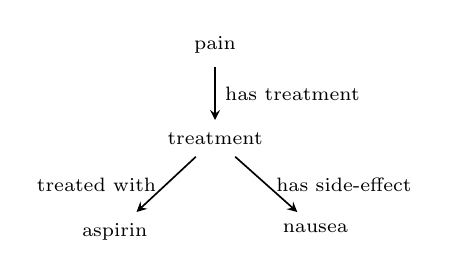
\begin{tikzpicture}[semithick, font = \scriptsize, draw = black, -stealth, shorten < = 1pt, shorten > = 1pt]
  \node (pain) {pain};
  \node (treatment) [below = 0.75cm of pain] {treatment};
  \node (aspirin) [below left = 0.75cm and 0cm of treatment] {aspirin};
  \node (nausea) [below right = 0.75cm and 0cm of treatment] {nausea};

  \draw (pain) -- node [midway, right] {has treatment} (treatment);
  \draw (treatment) -- node [midway, left] {treated with} (aspirin);
  \draw (treatment) -- node [midway, right] {has side-effect} (nausea);
\end{tikzpicture}

      \end{figure}
    \item Similarity measures may give better results, transparency, and explainabilty.
  \end{itemize}
\end{frame}

{\aauwavesbg%
\begin{frame}[plain, noframenumbering]
  \finalpage{Thank you!}
\end{frame}}

\end{document}
